% ==============================================================================
% CHAPITRE 1 : INTRODUCTION & CONTEXTE DU PROJET
% ==============================================================================

\chapter{Introduction et Contexte du Projet}
\label{ch:intro}

\section{Problématique : Détection des réseaux de blanchiment en continu}

Le blanchiment d'argent consiste à injecter des capitaux d'origine illicite dans le système financier légal tout en dissimulant leur provenance. Les criminels organisent ces flux selon trois étapes classiques :
\begin{enumerate}
    \item \textbf{Le Placement :} Introduction initiale des fonds en espèces dans le circuit bancaire (dépôts fractionnés ou \textit{smurfing}) ;
    \item \textbf{L'Empilement (\textit{Layering}) :} Multiplication rapide de virements entre plusieurs comptes intermédiaires (comptes mules) pour brouiller l'audit comptable et rompre le lien avec l'émetteur d'origine ;
    \item \textbf{L'Intégration :} Récupération des fonds apparemment régularisés pour investir dans l'économie légale.
\end{enumerate}

\begin{figure}[htbp]
    \centering
    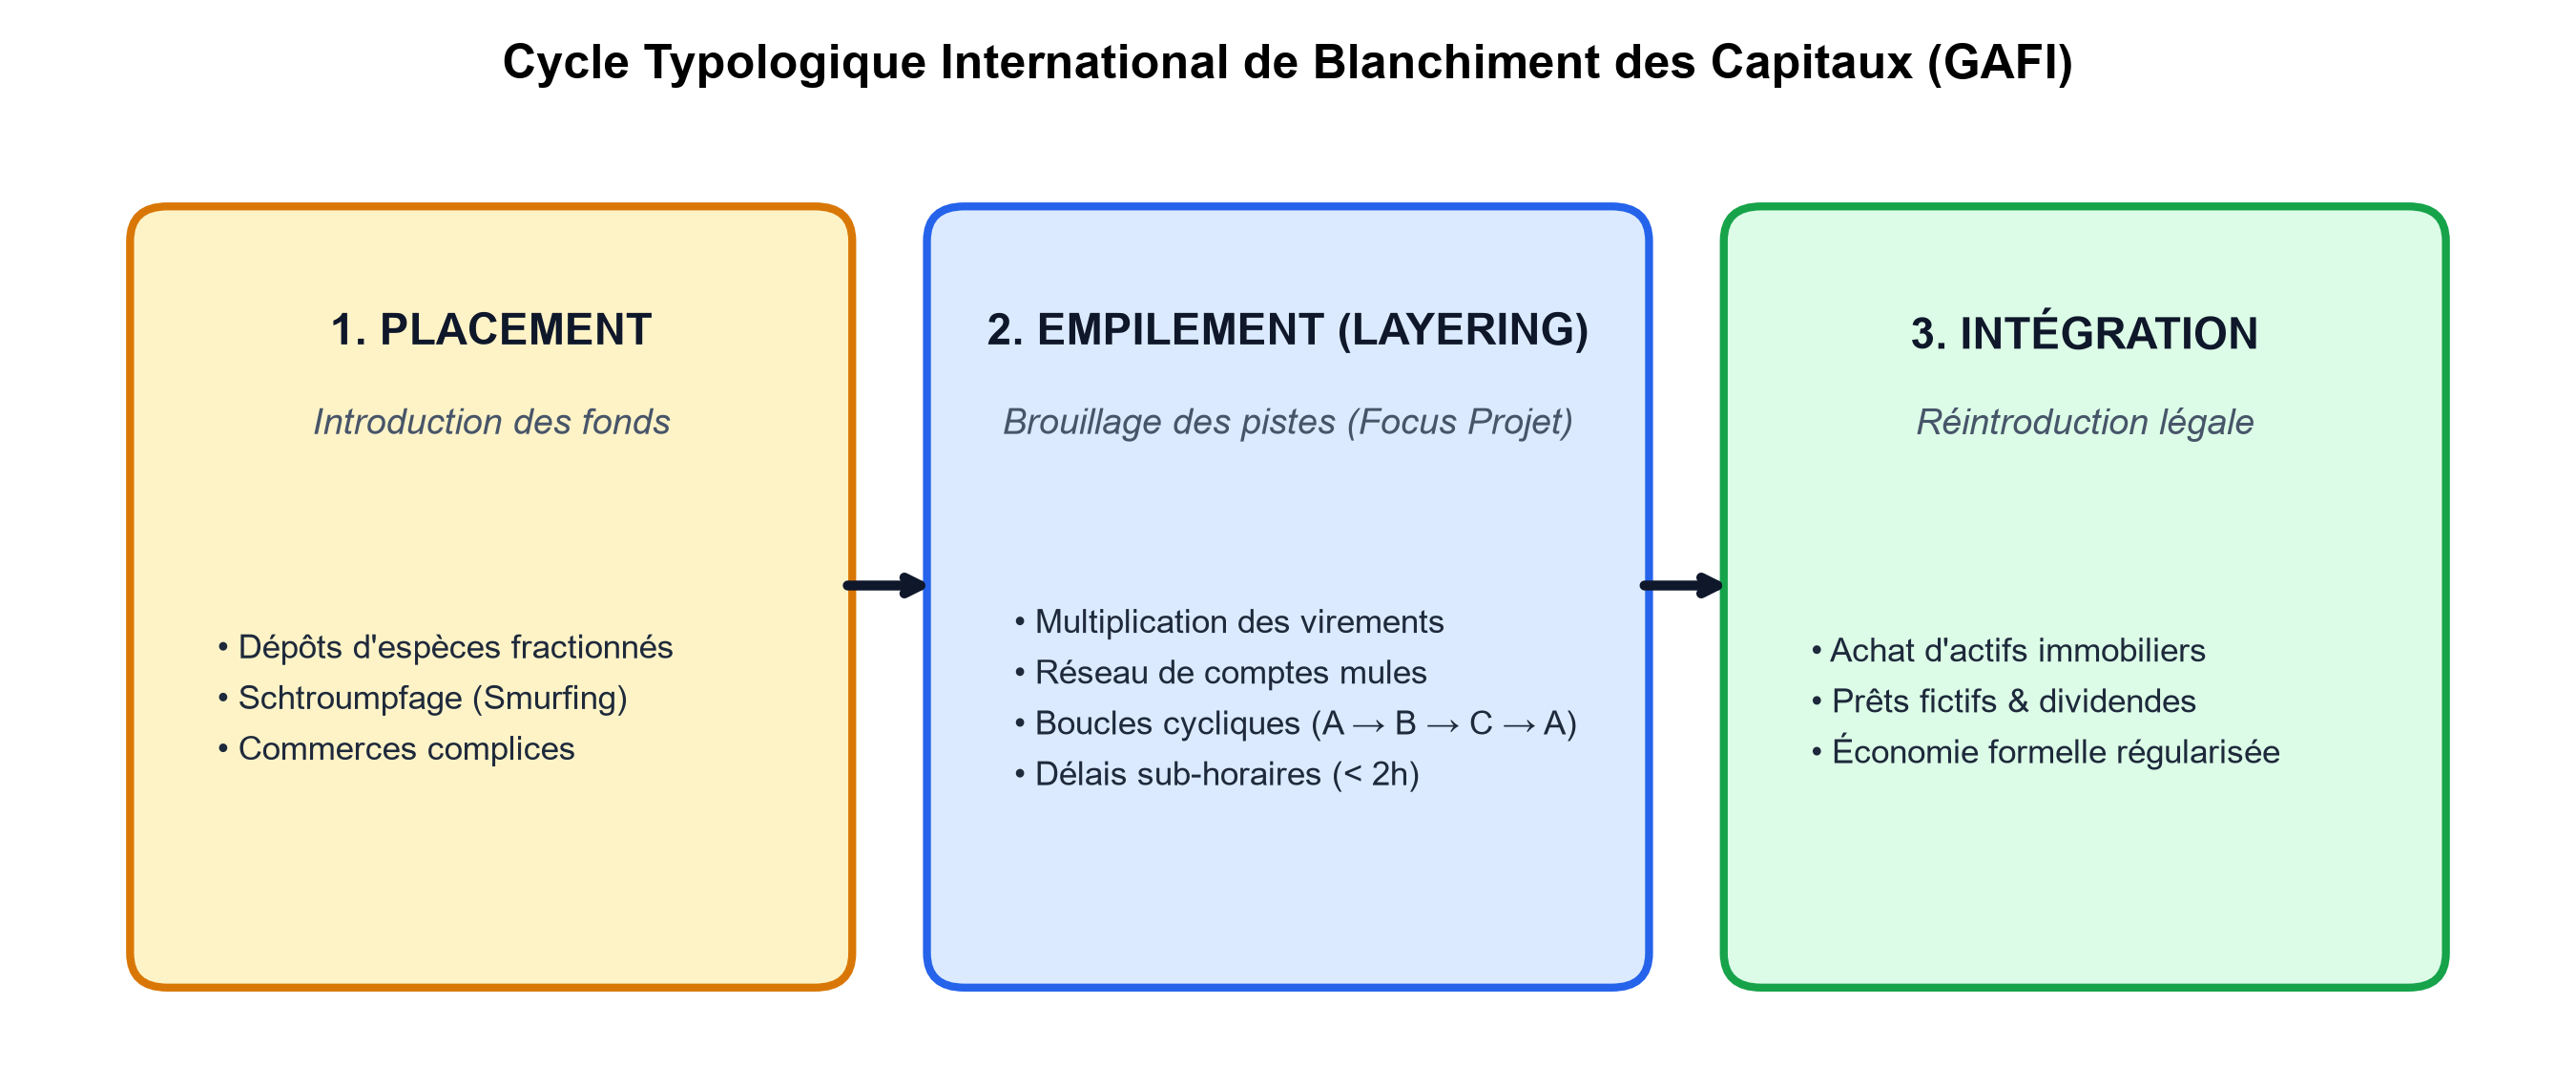
\includegraphics[width=0.92\linewidth]{figures/fig_placement_layering_integration.png}
    \caption{Les trois phases cardinales du blanchiment d'argent : Placement, Empilement (\textit{Layering}) et Intégration}
    \label{fig:aml_three_stages}
\end{figure}

Notre projet se focalise sur l'étape critique de l'\textbf{empilement}, et plus particulièrement sur la détection des **boucles circulaires fermées** (\textit{circular transaction loops}) où les fonds circulent selon un cycle orienté $A \to B \to C \to A$ dans un intervalle de temps court (moins de 2 heures) avec une déperdition minimale (commissions des complices inférieures à $15\,\%$).

\section{Limites des approches relationnelles conventionnelles}

Les systèmes bancaires traditionnels surveillent les transactions au moyen de requêtes SQL sur des bases de données relationnelles (SGBDR) et de règles tabulaires statiques (ex. alerter tout transfert supérieur à $100\,000\text{ MAD}$). Ces méthodes présentent trois faiblesses majeures :
\begin{itemize}
    \item \textbf{Explosion combinatoire des jointures :} Détecter un cycle à 3 nœuds en SQL impose plusieurs auto-jointures (\texttt{JOIN}) croisées sur une table de transactions comptant plusieurs millions de lignes, ce qui sature la mémoire du serveur ;
    \item \textbf{Traitement différé trop tardif :} Les analyses SQL s'exécutent généralement par lots la nuit (traitement batch à J+1). Or, les réseaux criminels vident et clôturent les comptes mules en quelques minutes après la fermeture de la boucle ;
    \item \textbf{Taux excessif de fausses alertes :} Les règles de montants bruts alertent indistinctement sur des commerces légitimes (supermarchés, stations-service) qui reçoivent naturellement un volume important de transferts.
\end{itemize}

\section{Objectifs et périmètre du projet}

L'objectif de ce projet est de concevoir et réaliser une plateforme de détection distribuée, capable d'ingérer les transactions en flux continu et d'isoler les boucles criminelles en temps réel à l'échelle du sous-graphe financier.

Le système développé s'articule autour de cinq briques techniques :
\begin{enumerate}
    \item Un bus de messages distribué \textbf{Apache Kafka} en mode KRaft pour l'ingestion des flux transactionnels ;
    \item Un moteur de calcul de flux \textbf{Apache Spark Structured Streaming} maintenant des fenêtres glissantes de $10\text{ minutes}$ et un filigrane de tolérance au retard de $120\text{ secondes}$ ;
    \item Le moteur de graphes \textbf{GraphFrames} pour exécuter les requêtes de motifs cycliques et recalculer périodiquement les métriques de centralité PageRank ;
    \item Un stockage transactionnel ACID \textbf{Delta Lake} pour historiser les données (Bronze, Silver, Gold) et garantir l'idempotence des alertes via un hachage canonique SHA-256 ;
    \item Une application web d'investigation en \textbf{Next.js 14} offrant un visualiseur de graphe interactif et l'exportation des dossiers réglementaires SAR au format JSON.
\end{enumerate}

\section{Organisation du document}

Le présent rapport est structuré comme suit :
Le Chapitre~\ref{ch:state_of_art} détaille les choix technologiques et les fondements théoriques (graphes, streaming et PageRank).
Le Chapitre~\ref{ch:architecture} décrit l'architecture système globale, les spécifications fonctionnelles et la structure des tables Delta Lake.
Le Chapitre~\ref{ch:streaming} expose l'implémentation du pipeline de streaming, de la validation des données à l'extraction des cycles.
Le Chapitre~\ref{ch:dashboard} présente le tableau de bord d'investigation médico-légale développé en Next.js.
Le Chapitre~\ref{ch:experiments} détaille la validation sur le jeu de données IBM AMLSim, la matrice des 22 tests d'acceptation et les benchmarks de charge.
Enfin, le Chapitre~\ref{ch:conclusion} conclut le mémoire et présente les perspectives d'évolution.
